\documentclass[14pt]{extarticle}
% Full article preamble (duplicated, no common file)
\usepackage{fontspec}
\usepackage[a4paper,top=2.4cm,bottom=2.4cm,left=2.3cm,right=2.3cm]{geometry}
\usepackage{polyglossia}
\usepackage{amsmath}
\usepackage{amssymb}
\usepackage{xcolor}
\usepackage{fancyhdr}
\usepackage{graphicx}
\usepackage{listings}
\usepackage[most]{tcolorbox}
\usepackage{pifont}
\usepackage{enumitem}
\usepackage{titlesec}
\usepackage[bottom]{footmisc}
\usepackage{titling}
\usepackage{minted}
\usepackage{etoolbox}
\usepackage{array}
\usepackage{extsizes}

\newfontfamily\emoji{Segoe UI Emoji}

\pagestyle{fancy}

\setmainlanguage[numerals=western]{arabic}
\setotherlanguage{english}
\newfontfamily\arabicfont[Script=Arabic]{Amiri}
\newfontfamily\arabicfonttt[Script=Arabic]{Courier New}

\lstset{
  language=[Sharp]C,
  numbers=left,
  stepnumber=1,
  numbersep=8pt,
  frame=single,
  basicstyle=\ttfamily\small,
  keywordstyle=\color{blue},
  stringstyle=\color{red},
  commentstyle=\color{green!50!black}
}

\newif\ifdetailed
\ifdefined\setdetailed
  \setdetailed
\fi

\newif\ifwithsols
\ifdefined\setwithsols
  \setwithsols
\fi

% unified tcolorboxes for articles
\tcbset{colback=white, colframe=black, fonttitle=\bfseries, boxrule=0.8pt}
\newtcolorbox{boxDef}[1][]{colback=blue!5!white,colframe=blue!75!black,
  title={{\emoji📘} تعريف\ifx\\#1\\\else ~#1\fi :}}
\newtcolorbox{boxExercise}[1][]{colback=cyan!5!white,colframe=cyan!70!black,
  title={{\emoji🧩} تمرين\ifx\\#1\\\else ~#1\fi :}}
\newtcolorbox{boxExample}[1][]{colback=yellow!5!white,colframe=orange!90!black,
  title={{\emoji📝} مثال\ifx\\#1\\\else ~#1\fi :}}
\newtcolorbox{boxNote}[1][]{colback=gray!10!white,colframe=black,
  title={{\emoji✨} ملاحظة\ifx\\#1\\\else ~#1\fi :}}
\newtcolorbox{boxAttention}[1][]{colback=magenta!10!white,colframe=magenta!80!black,
  title={{\emoji🔔} تنبيه\ifx\\#1\\\else ~#1\fi :}}
\newtcolorbox{boxWarning}[1][]{colback=red!5!white,colframe=red!75!black,
  title={{\emoji⚡} ملاحظة هامة\ifx\\#1\\\else ~#1\fi :}}
\newtcolorbox{boxSolution}[1][]{colback=green!5!white,colframe=green!60!black,
  title={{\emoji✅} حل\ifx\\#1\\\else ~#1\fi :}}
\newtcolorbox{boxSymbol}[1][]{colback=purple!5!white,colframe=purple!70!black,
  title={{\emoji🔣} رمز\ifx\\#1\\\else ~#1\fi :}}
\newtcolorbox{boxHint}[1][]{colback=teal!5!white,colframe=teal!60!black,
  title={{\emoji💡} تلميح\ifx\\#1\\\else ~#1\fi :}}


\tcbset{simplecode/.style={ colback=gray!5, colframe=black!50, boxrule=0.4pt, arc=2pt, left=4pt,right=4pt,top=4pt,bottom=4pt}}
\newenvironment{boxCode}{\begin{tcolorbox}[simplecode]}{\end{tcolorbox}}

\newcolumntype{C}[1]{>{\centering\arraybackslash}p{#1}}

% redefine spaces after titles
\makeatletter
\renewcommand{\@maketitle}{%
  \begin{center}
    {\huge \bfseries \@title \par}%
    \vskip 0.2em % space between title and author
    {\large \@author \par}%
    % \vskip 0.2em % space between author and date
    % {\normalsize \@date \par}%
  \end{center}
}
\makeatother

\fancyhf{} % clear default
\fancypagestyle{plain}{
  \fancyhf{}
  \fancyhead[L]{مدرسة التسامح الشاملة}
  % \fancyhead[L]{\includegraphics[height=1cm]{../../../images/logoTasamoh.png}}
  \fancyhead[R]{الأستاذ محمود اغبارية}
  \fancyfoot[C]{\thepage}
}

\fancyhead[L]{مدرسة التسامح الشاملة}
\fancyhead[R]{الأستاذ محمود اغبارية}
\fancyfoot[C]{\thepage}
% \date{\today}

\setcounter{tocdepth}{3} % only section subsection and subsubsection in TOC


% ----------------------


% \begin{document}

% \maketitle

% % \clearpage  % start TOC on a new page
% % \renewcommand{\contentsname}{جدول المحتويات}
% % \tableofcontents
% % \clearpage

% \part*{part 1} % the * prevents numbering
% \section*{مقدمة}
% \subsection*{مثال رياضي}
% \subsubsection*{مثال فرعي}
% \paragraph*{ paragraph 1}
% \subparagraph*{sub paragraph 1}

% \ifdetailed
% \begin{english}
% \begin{minted}{csharp}
% // C# Example
% \end{minted}
% \end{english}
% \fi

% OLD WAY
% \ifdetailed
% \begin{english}
% \begin{lstlisting}
% // C# Example
% \end{lstlisting}
% \end{english}
% \fi

% % \includegraphics[width=0.2\textwidth]{../../../images/DFAs/ex1_q1.png}



% \vspace{3cm}
% \begin{flushleft}
% أرجو لكم وقتًا ممتعًا.

% الأستاذ محمود اغبارية.
% \end{flushleft}


% \end{document}


\begin{document}

\pagestyle{empty}
\thispagestyle{empty}

\section*{الفصل الثاني}

\textbf{أجب عن السؤالين 3 و 4.}

\begin{enumerate}[itemsep=3em, start=3, label=\arabic*)]

\item
معطاة اللغة $L$ فوق الأبجدية $\{a,b\}$: \\
$=L$ كل الكلمات التي طولها فردي، وأيضًا لا تحتوي على السلسلة $aba$.

\begin{enumerate}[label=\alph*., itemsep=2em]
    \item أمامكم خمس كلمات:
    $ ababa, \ \ b, \ \ aa, \ \ bab, \ \ abb $
    انسخوا كلّ واحدة من الكلمات إلى دفتركم، وحدّدوا إذا كانت تتبع للغة $L$ أم لا تتبع للغة $L$. علّلوا تحديداتكم.
\ifwithsols
\begin{boxSolution}
\begin{itemize}
    \item $ababa$: لا تتبع للغة $L$، لأنّها تحتوي على السلسلة $aba$
    \item $b$: تتبع للغة $L$، طولها فردي ولا تحتوي على $aba$.
    \item $aa$: لا تتبع للغة $L$، طولها زوجي.
    \item $bab$: تتبع للغة $L$، طولها فردي ولا تحتوي على $aba$.
    \item $abb$: تتبع للغة $L$، طولها فردي ولا تحتوي على $aba$.
\end{itemize}
\end{boxSolution}
\clearpage
\fi

    \item معطى أمامكم في الرسم أدناه تخطيط لأوتومات نهائيّ محدود \textbf{كامل} يتلقّى اللغة $L$.
    يحتوي التخطيط على جميع الحالات وجميع الأسهم اللازمة، لكن تنقص \textbf{إشارات الإدخال} (الحروف $a$ أو $b$ بجانب الأسهم)، \textbf{والحالات المتلقية}

\begin{center}
    \includegraphics[width=0.9\textwidth]{../../../images/DFAs/odd_length_no_aba_withoutTransitions.png}
\end{center}

انسخوا الأوتومات إلى دفتركم، أضيفوا إشارات الإدخال الناقصة على الأسهم، وأشيروا بدائرة مزدوجة إلى الحالات المتلقّية.

\ifwithsols
\begin{boxSolution}
\begin{center}
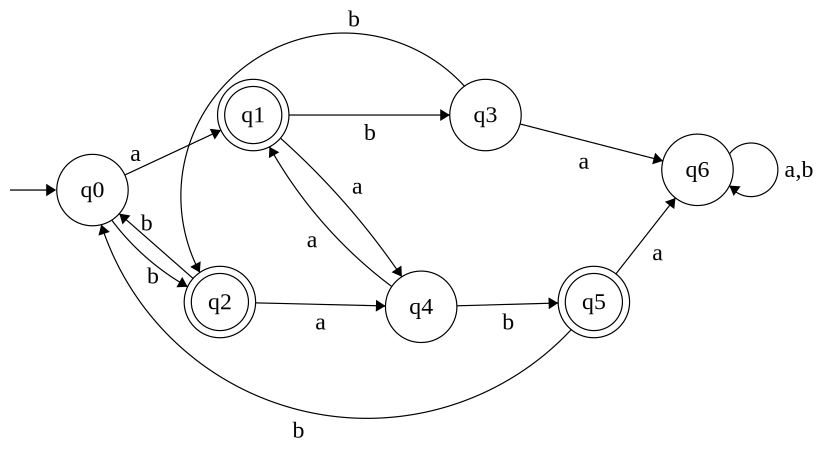
\includegraphics[width=\textwidth]{../../../images/DFAs/odd_length_no_aba.png}
\end{center}
\end{boxSolution}
\fi
\end{enumerate}

\clearpage
\item
في هذا السؤال بندان، "أ-ب"، لا علاقة بينهما. أجيبوا عن البندين.


\begin{enumerate}[label=\alph*., itemsep=2em]
    \item
معطاة لغتان نظاميّتان، $L_1$ و $L_2$، فوق الأبجدية $\Sigma$. \\
نُعرّف اللغة الجديدة $L_{new}$ بالشكل التالي:
$$L_{new} = \{ w \in \Sigma^* \mid R(w) \in L_1 \textbf{ وأيضًا } w \notin L_2 \}$$
برهنوا أنّ اللغة $L_{new}$ هي لغة نظاميّة. اعتمدوا في برهانكم على صفات الانغلاق للغات النظامية.
\ifwithsols
\begin{boxSolution}
يمكننا التعبير عن اللغة $L_{new}$ بالطريقة التالية:
اللغة $L_{new} = R(L_1) \cap \overline{L_2}$. \\

اللغات النظامية مغلقة تحت عملية المقلوب، والمكمل، والتقاطع. \\
بما أن $L_1$ و $L_2$ نظاميتان، فإن $R(L_1)$ و $\overline{L_2}$ نظاميتان، وبالتالي تقاطعهما $L_{new}$ نظامية.
\end{boxSolution}
\clearpage
\fi

\item
أمامك اللغات $L_1, L_2, L_3$ فوق الأبجدية $\{a,b\}$
\begin{align*}
L_1 &= \{w \mid aba \text{ تحتوي التسلسل } w\} \\
L_2 &= \{w \mid \text{ تبدأ وتنتهي بنفس الرمز} w\} \\
L_3 &= \{w \mid \#_a(w) = 2 \times \#_b(w) \}
\end{align*}
بالنسبة لكل واحد من الادعاءات التالية، حدّد إذا كان صحيحًا أم غير صحيح. \\
إذا كان الادعاء صحيحًا — فسّر لماذا. \\
وإذا كان الادعاء غير صحيح — فسّر لماذا أو أعطِ مثالًا يدحض الادعاء، وفسّر لماذا يدحضه.
\begin{enumerate}[label=\textbf{(\arabic*)}, itemsep=1em]
    \item $aabaa \in L_1 \cup L_3$
    \item $L_2 = R(L_2)$
    \item $\overline{L_3} = \{w \mid 2 \times \#_a(w) = \#_b(w) \}$
    \item $\epsilon \in \overline{L_1} \cap L_3$
    \item $L_1 \cap L_2 \cap L_3 = \emptyset$
    \item $L_1 \cdot L_3 \subseteq L_3$
\end{enumerate}
\ifwithsols
\begin{boxSolution}
\begin{enumerate}[label=\textbf{(\arabic*)}, itemsep=1em]
    \item صحيح، لأن $aabaa$ تحتوي على $aba$، فهي في $L_1$.
    \item صحيح، لأن اللغة $L_2$ تحتوي على الكلمات التي تبدأ وتنتهي بنفس الرمز، وهذه الخاصية تظل صحيحة تحت العملية العكسية.
    \item غير صحيح، اللغة المكملة لـ $L_3$ هي لغة كل الكلمات التي لا يتحقق فيها أنّ $\#_a(w) = 2 \times \#_b(w)$. \\
مثلًا: الكلمة $ab$ ليست موجودة في اللغة $L_3$، لذلك يجب أن تكون موجودة في $\overline{L_3}$ ، لكنها ليست موجودة في اللغة الموصوفة: $2 \times \#_a(w) = \#_b(w)$ لذلك لا يمكن أن تكون هذه هي $\overline{L_3}$.
    \item صحيح، لأن $\epsilon \notin L_1$ (لا تحتوي على $aba$)، لذلك: $\epsilon \in \overline{L_1}$. \\
و $\#_a(\epsilon) = 0 = 2 \times 0$. لذلك: $\epsilon \in L_3$ \\
لذلك $\epsilon \in \overline{L_1} \cap L_3$ لأنه موجود في كليهما.
    \item غير صحيح، مثال: $aba \in L_1 \cap L_2 \cap L_3$، لأنها تحتوي على $aba$، تبدأ وتنتهي بـ $a$، و $\#_a=2$، $\#_b=1$، $2 = 2 \times 1$.
    \item
غير صحيح، مثلًا: الكلمة  $w_1 = baba \in L_1$ والكلمة $w_2 = aba \in L_3$، عندها: $w_1 \cdot w_2 = babaaba$ وهذه الكلمة ليست موجودة في $L_3$ لأنّ عدد الـ $a$ فيها ليس ضعف عدد الـ $b$.
\end{enumerate}
\end{boxSolution}
\fi

\end{enumerate}

\end{enumerate}

% \vspace{1cm}
\begin{flushleft}
نرجو لكم التفوّق.

معلمو الموضوع.
\end{flushleft}

\end{document}
